\section{Short Runs}

\subsection{Stochastic Loads Method}
This solution was run with a targeted execution time of approximately 7-8 minutes. The solution was calculated using the following command line arguments to the solver: 

\begin{verbatim}
python -m pystruct <<data_file>>  -S3 -i30 -g25 --csv
\end{verbatim}

\noindent Where: 

\begin{itemize}
  \item \codeword{-S3}: Select solution 3: Stochastic Loads Method
  \item \codeword{-i30}: Use a population size of 30. 
  \item \codeword{-g25}: Use a generation count of 25. 
  \item \codeword{--csv}: Generate CSV output for final Pareto Front
\end{itemize}


\subsubsection{Resultant Pareto Front}
Table \ref{tab:pfront_sto_short} shows the design parameters of the members of the Pareto Front generated by this solution run. The Pareto Front is also given graphically in Figure \ref{fig:pfront_sto_short}. 

\begin{table}[!htbp]
\centering
\small
\begin{tabular}{|p{1.5cm}p{1.5cm}p{1.4cm}p{2cm}p{2cm}||p{1.5cm}p{1.5cm}|}
\hline
\multicolumn{5}{|c||}{Design Parameters}&\multicolumn{2}{|c|}{Fitness Properties}\\
\hline
Top Flange Width&Bottom Flange Width&Web Thickness&Doubler Thickness at Hoist Pin&Doubler Thickness at Load Pin&Reliability Index& Mass\\
\hline
mm&mm&mm&mm&mm&ul&kg\\
\hline
170.039&245.14&71.477&192.605&189.368&6.578&929.701\\
61.042&223.528&106.182&54.387&103.309&6.651&990.429\\
248.513&224.849&77.891&30.268&54.893&6.473&816.670\\
197.478&184.497&17.633&92.008&136.953&5.407&414.890\\
103.886&16.745&16.36&158.441&185.596&2.562&372.892\\
230.115&176.491&20.515&21.348&203.78&5.562&419.033\\
43.425&101.887&53.24&200.759&78.852&5.628&645.181\\
143.639&222.302&73.671&32.004&87.213&6.437&757.066\\
\hline
\end{tabular}
	\caption{Members of the Pareto Front generated through Stochastic Loads (Short Run)}
\label{tab:pfront_sto_short}
\end{table}

\begin{figure}
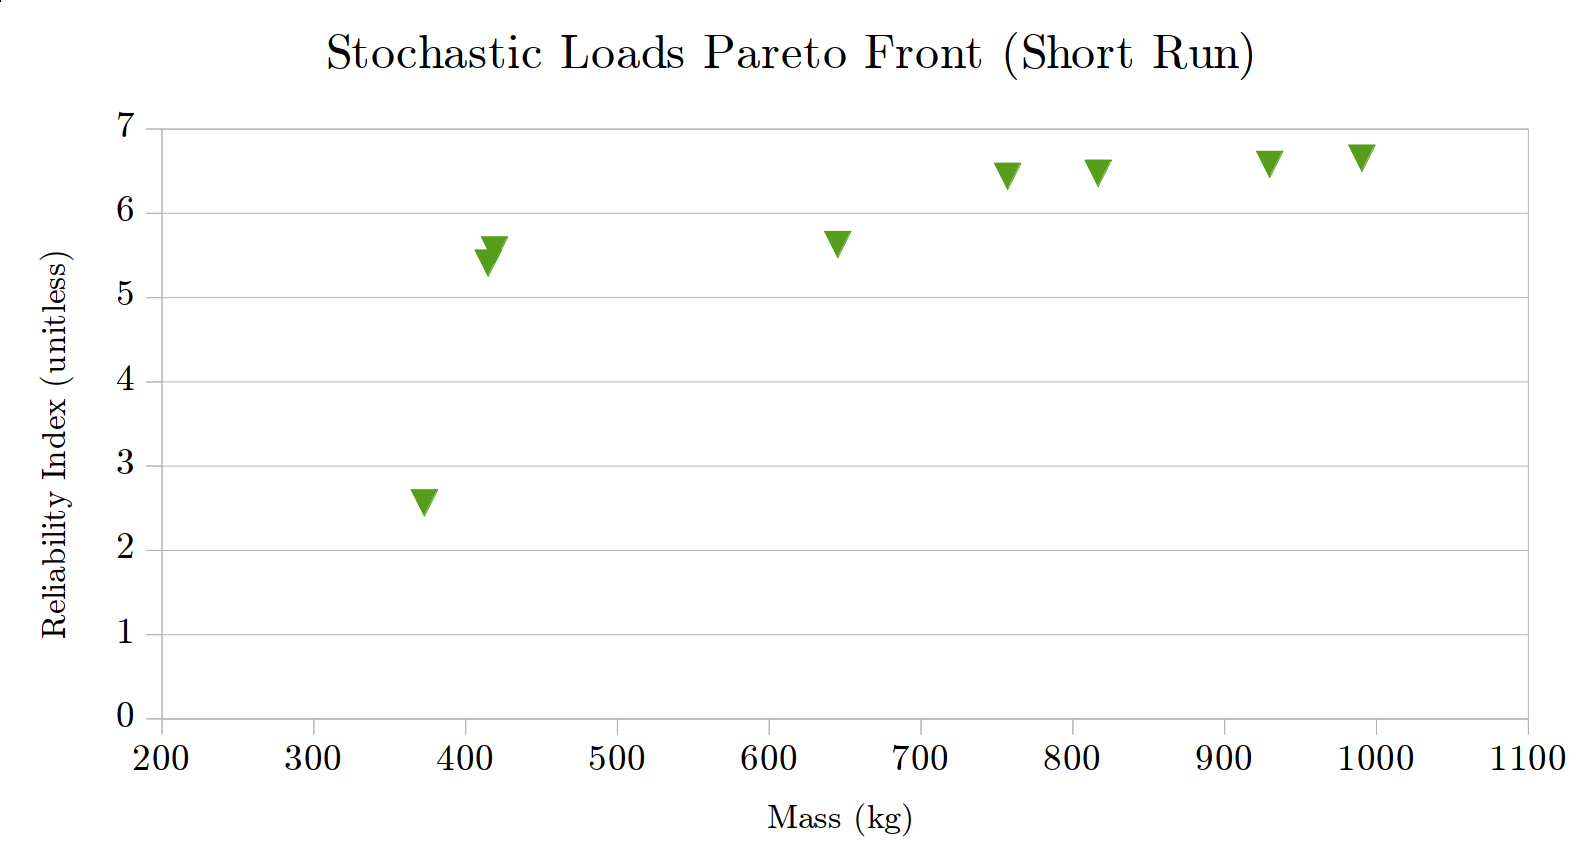
\includegraphics[width=\textwidth]{img/pf_sto_short.png}
	\caption{Graph of the Pareto Front generated through Stochastic Loads (Short Run)}
\label{fig:pfront_sto_short}
\end{figure}

\subsubsection{Solution Statistics}
This solution also was tracked for several computing performance indicators to compare the performance of the algorithm with the other solutions. These statistics are listed in Table \ref{tab:stat_sto_short}. 

\begin{table}[!htbp]
  \centering
  \begin{tabular}{|l|l|}
    \hline
	  Total Generations Computed & 25\\
    Average Time Per Generation (sec) & 18.1\\
    Total Wall Clock Time (sec)	 & 453\\
    \hline
  \end{tabular}
	\caption{Solution Statistics for Stochastic Loads (Short Run)}
  \label{tab:stat_sto_short}
\end{table}

\subsection{Aggregate LHS Method}
This solution was calculated using parameters designed to produce approximately the same wall clock solution time as the Stochastic Loads Short Run above. The command line that was used was:

\begin{verbatim}
python -m pystruct <<data_file>>  -S2 -i20 -g2 --csv
\end{verbatim}

\noindent Where: 

\begin{itemize}
  \item \codeword{-S2}: Select solution 2: Aggregate LHS method
  \item \codeword{-i20}: Use a population size of 20. 
  \item \codeword{-g2}: Use a generation count of 2. 
  \item \codeword{--csv}: Generate CSV output for final Pareto Front
\end{itemize}

\subsubsection{Resultant Pareto Front}
Table \ref{tab:pfront_agg_short} shows the design parameters of the members of the Pareto Front generated by this solution run. The Pareto Front is also given graphically in Figure \ref{fig:pfront_agg_short}. 
\begin{table}[!htbp]
\small
\begin{tabular}{|p{1.5cm}p{1.5cm}p{1.5cm}p{1.4cm}p{2cm}p{2cm}||p{1.5cm}p{1.5cm}|}
\hline
\multicolumn{6}{|c||}{Design Parameters}&\multicolumn{2}{|c|}{Fitness Properties}\\
\hline
Parent Load Case&Top Flange Width&Bottom Flange Width&Web Thickness&Doubler Thickness at Hoist Pin&Doubler Thickness at Load Pin&Peak Stress& Mass\\
\hline
&mm&mm&mm&mm&mm&MPa&kg\\
\hline
5&129.488&178.7&50.012&64.189&66.968&65.185&574.583\\
6&49.705&155.799&78.425&32.802&132.61&52.474&747.643\\
6&151.264&247.119&22.268&102.256&62.329&73.893&432.479\\
6&99.534&146.74&64.76&52.983&244.566&53.820&725.557\\
7&142.734&225.029&57.877&144.821&224.451&49.166&786.819\\
8&74.907&224.589&54.305&48.5&59.581&61.755&587.581\\
10&215.954&234.061&88.335&55.669&231.921&38.577&979.637\\
11&140.513&241.439&18.337&53.885&203.955&80.989&418.511\\
12&178.503&194.828&43.687&147.502&187.016&59.195&669.831\\
12&206.098&236.439&75.92&91.15&157.782&42.924&880.824\\
12&160.811&167.923&69.169&134.097&230.611&48.597&849.269\\
13&81.25&202.425&42.572&109.538&81.68&67.260&551.180\\
17&23.721&163.915&49.492&31.35&127.582&72.366&522.037\\
18&140.976&128.319&39.838&34.495&234.181&72.149&530.609\\
18&102.296&214.843&13.829&47.973&164.341&89.932&337.531\\
18&49.437&171.257&79.644&147.498&193.402&48.320&878.472\\
19&54.821&251.784&24.932&117.632&33.267&86.715&415.135\\
22&52.03&186.161&10.735&57.554&199.908&118.283&305.286\\
\hline
\end{tabular}
\caption{Members of the Pareto Front generated through Aggregated LHS (Short Run)}
\label{tab:pfront_agg_short}
\end{table}

\begin{figure}[!htbp]
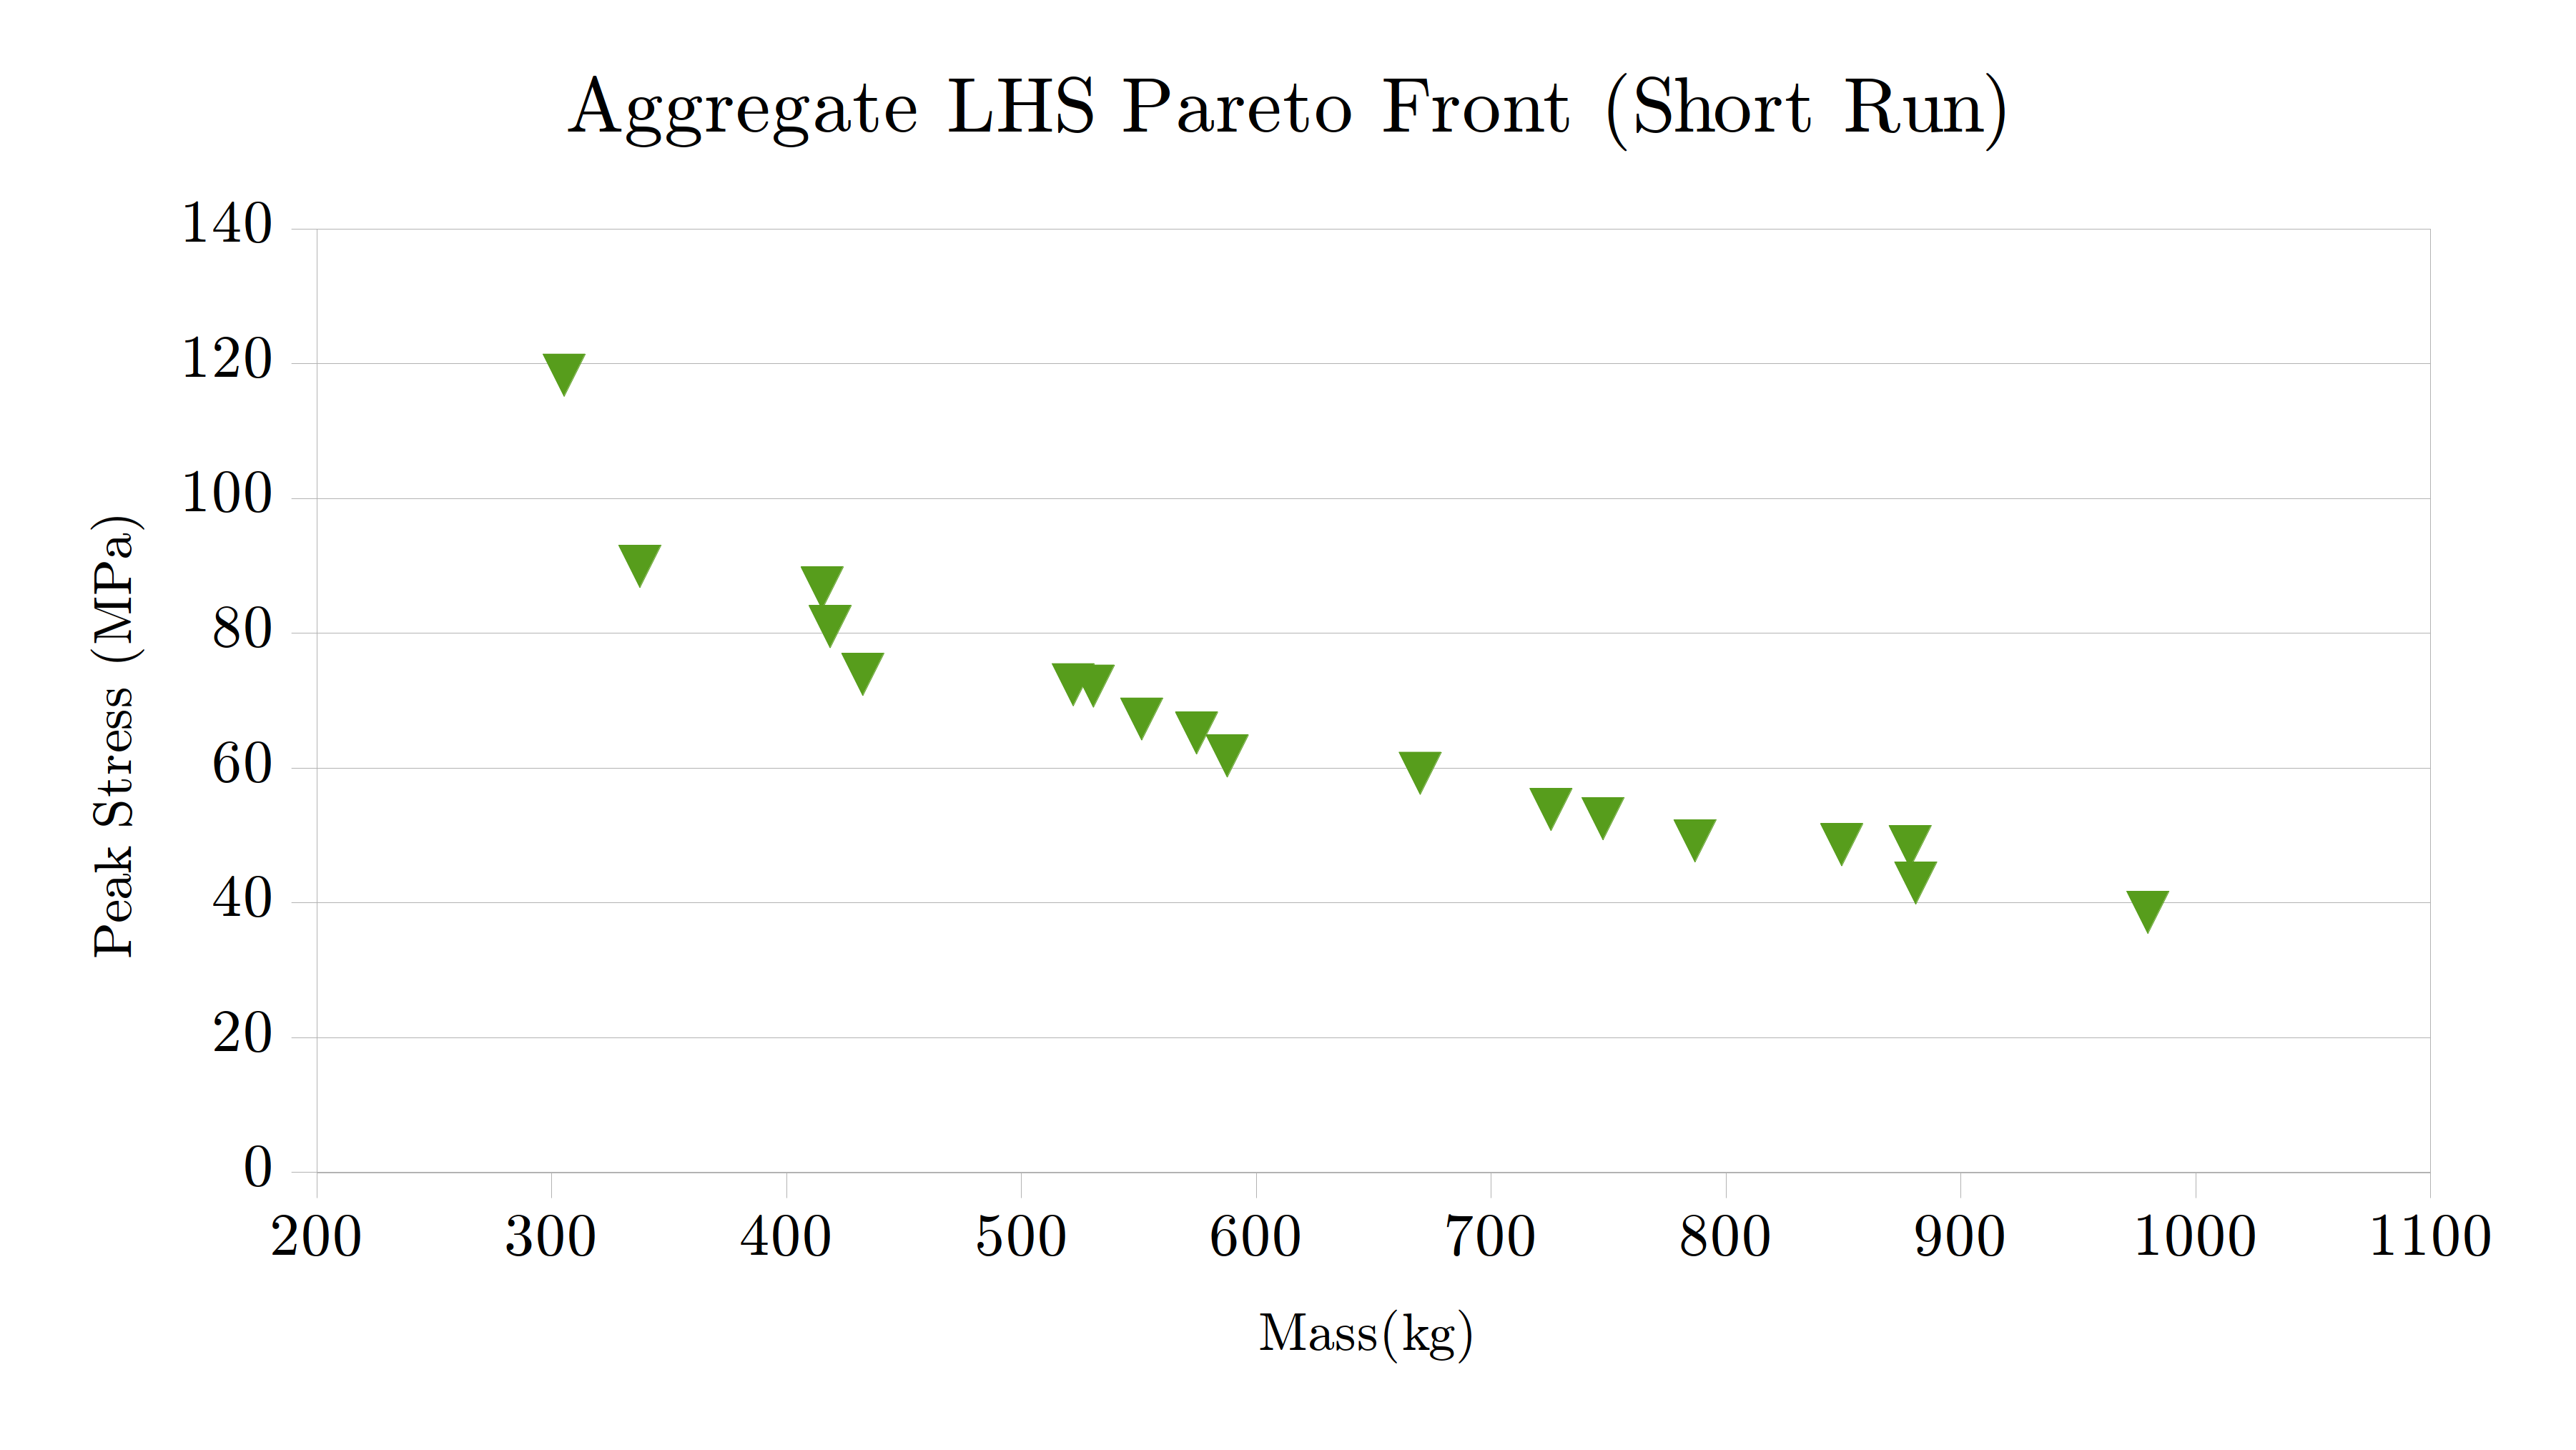
\includegraphics[width=\textwidth]{img/pf_agg_short.png}
\caption{Graph of the Pareto Front generated through Aggregated LHS (Short Run)}
\label{fig:pfront_agg_short}
\end{figure}

\subsubsection{Solution Statistics}
This solution also was tracked for several computing performance indicators to compare the performance of the algorithm with the other solutions. These statistics are listed in Table \ref{tab:stat_agg_short}. 

\begin{table}[!htbp]
  \centering
  \begin{tabular}{|l|l|}
    \hline
	  Total Generations Computed & 50\\
    Average Time Per Generation (sec) & 8.22\\
    Total Wall Clock Time (sec)	 & 411\\
    \hline
  \end{tabular}
\caption{Solution Statistics for Aggregated LHS (Short Run)}
  \label{tab:stat_agg_short}
\end{table}

